% Created 2023-11-14 Tue 08:30
% Intended LaTeX compiler: pdflatex
\documentclass[11pt]{article}
\usepackage[utf8]{inputenc}
\usepackage[T1]{fontenc}
\usepackage{graphicx}
\usepackage{longtable}
\usepackage{wrapfig}
\usepackage{rotating}
\usepackage[normalem]{ulem}
\usepackage{amsmath}
\usepackage{amssymb}
\usepackage{capt-of}
\usepackage{hyperref}
\graphicspath{{../../books/}}
% TIPS
% \substack{a\\b} for multiple lines text





% pdfplots will load xolor automatically without option
\usepackage[dvipsnames]{xcolor}

\usepackage{forest}
% two-line text in node by [two \\ lines]
% \begin{forest} qtree, [..] \end{forest}
\forestset{
  qtree/.style={
    baseline,
    for tree={
      parent anchor=south,
      child anchor=north,
      align=center,
      inner sep=1pt,
    }}}
%\usepackage{flexisym}
% load order of mathtools and mathabx, otherwise conflict overbrace

\usepackage{mathtools}
%\usepackage{fourier}
\usepackage{pgfplots}
\usepackage{amsthm, mathabx,  amsmath, commath}
\usepackage{amsfonts}

\usepackage{empheq}
\usepackage{tikz}
\usetikzlibrary{arrows.meta}
\usepackage[most]{tcolorbox}

\newtheorem{theorem}{Theorem}[section]
\newtheorem{definition}{Definition}[section]
\newtheorem{corollary}{Corollary}[section]
\newtheorem{example}{Example}[section]
\newtheorem{lemma}{Lemma}[section]
\newtheorem{proposition}{Proposition}[section]

\newcommand{\bl}[1] {\boldsymbol{#1}}
\newcommand{\Wt}[1] {\stackrel{\sim}{\smash{#1}\rule{0pt}{1.1ex}}}
\newcommand{\wt}[1] {\widetilde{#1}}


%For boxed texts in align, use Aboxed{}
%otherwise use boxed{}

\DeclareMathSymbol{\widehatsym}{\mathord}{largesymbols}{"62}
\newcommand\lowerwidehatsym{%
  \text{\smash{\raisebox{-1.3ex}{%
    $\widehatsym$}}}}
\newcommand\fixwidehat[1]{%
  \mathchoice
    {\accentset{\displaystyle\lowerwidehatsym}{#1}}
    {\accentset{\textstyle\lowerwidehatsym}{#1}}
    {\accentset{\scriptstyle\lowerwidehatsym}{#1}}
    {\accentset{\scriptscriptstyle\lowerwidehatsym}{#1}}
}

\usepackage{graphicx}
    
% text on arrow for xRightarrow
\makeatletter
%\newcommand{\xRightarrow}[2][]{\ext@arrow 0359\Rightarrowfill@{#1}{#2}}
\makeatother


\def \bx {\boldsymbol{x}}
\def \ba {\boldsymbol{a}}
\def \bI {\boldsymbol{I}}
\def \bt {\boldsymbol{t}}
\def \bb {\boldsymbol{b}}
\def \bA {\boldsymbol{A}}
\def \bX {\boldsymbol{X}}
\def \bu {\boldsymbol{u}}
\def \bS {\boldsymbol{S}}
\def \bZ {\boldsymbol{Z}}
\def \bz {\boldsymbol{z}}
\def \by {\boldsymbol{y}}
\def \bw {\boldsymbol{w}}
\def \bT {\boldsymbol{T}}
\def \bS {\boldsymbol{S}}
\def \bm {\boldsymbol{m}}
\def \bW {\boldsymbol{W}}
\def \bY {\boldsymbol{Y}}
\def \bH {\boldsymbol{H}}
\def \blambda {\boldsymbol{\lambda}}
\def \bPhi {\boldsymbol{\Phi}}
\def \btheta {\boldsymbol{\theta}}
\def \bmu {\boldsymbol{\mu}}
\def \bphi {\boldsymbol{\phi}}
\def \bSigma {\boldsymbol{\Sigma}}
\def \lb {\left\{}
\def \rb {\right\}}
\def \caln {\mathcal{N}}
\def \dissum {\displaystyle\Sigma}
\def \dispro {\displaystyle\prod}
\def \E {\mathbb{E}}
\def \Q {\mathbb{Q}}
\def \V {\mathbb{V}}
\def \R {\mathbb{R}}
\def \calq {\mathcal{Q}}
\def \calg {\mathcal{G}}
\def \caln {\mathcal{N}}
\def \calr {\mathcal{R}}
\def \calm {\mathcal{M}}
\def \calc {\mathcal{C}}
\def \bcup {\bigcup}

\makeindex
\author{Martin Kleppmann}
\date{\today}
\title{Designing Data-Intensive Applications}
\hypersetup{
 pdfauthor={Martin Kleppmann},
 pdftitle={Designing Data-Intensive Applications},
 pdfkeywords={},
 pdfsubject={},
 pdfcreator={Emacs 29.1 (Org mode 9.7)}, 
 pdflang={English}}
\begin{document}

\maketitle
\tableofcontents

\section{Storage and Retrieval}
\label{sec:org7bf51a4}

\subsection{Data Structures That Power Your Database}
\label{sec:org7158a46}

\subsubsection{Hash Indexes}
\label{sec:orgace6a7a}

\subsubsection{SSTables and LSM-Trees}
\label{sec:org1fb15ec}
\section{Replication}
\label{sec:org3fc2967}
\subsection{Leaders and Followers}
\label{sec:org21769ce}
\subsubsection{Setting Up New Followers}
\label{sec:orgfabea72}
\begin{enumerate}
\item Take a consistent snapshot of the leader's database at some point in time
\item Copy the snapshot to the new follower node
\item The follower connects to the leader and requests all the data changes that have happened
since the snapshot was taken. This requires that the snapshot is associated with an exact
position in the leader's replication log
\item When the follower has processed the backlog of data changes since the snapshot, we say it has
\textbf{caught up}
\end{enumerate}
\subsubsection{Handling Node Outages}
\label{sec:org520c0af}
\begin{enumerate}
\item Follower failure: Catch-up recovery
\label{sec:org9c19399}
\item Leader failure: Failover
\label{sec:orge9c6514}
\textbf{Failover}: one of the followers needs to be promoted to be the new leader, clients need to be
reconfigured to send their writes to the new leader, and the other followers need to start
consuming data changes from the new leader.
\begin{enumerate}
\item \emph{Determining that the leader has failed}.
\item \emph{Choosing a new leader}.
\item \emph{Reconfiguring the system to use the new leader}.
\end{enumerate}


Failover is fraught with things that can go wrong:
\begin{enumerate}
\item If asynchronous replication is used, the new leader may not have received all the writes from
the old leader before it failed. If the former leader rejoins the cluster after a new leader
has been chosen, what should happen to those writes? The new leader may have received
conflicting writes in the meantime. The most common solution is for the old leader’s
unreplicated writes to simply be \textbf{discarded}, which may violate clients' durability
expectations.
\item Discarding writes is especially dangerous if other storage systems outside of the database
need to be coordinated with the database contents. For example, in one incident at GitHub, an
out-of-date MySQL follower was promoted to leader. The database used an
autoincrementing counter to assign primary keys to new rows, but because the new leader’s
counter lagged behind the old leader’s, it reused some primary keys that were previously
assigned by the old leader. These primary keys were also used in a Redis store, so the reuse
of primary keys resul‐ ted in inconsistency between MySQL and Redis, which caused some
private data to be disclosed to the wrong users.
\item In certain fault scenarios, it could happen that two nodes both believe that they are the
leader. This situation is called \textbf{split brain}.
\item What is the right timeout before the leader is declared dead? A longer timeout means a longer
time to recovery in the case where the leader fails. However, if the timeout is too short,
there could be unnecessary failovers.
\end{enumerate}
\end{enumerate}
\subsubsection{Implementation of Replication Logs}
\label{sec:org2602c1b}
\begin{enumerate}
\item Statement-based replication
\label{sec:org2f44a5c}
In the simplest case, the leader logs every write request (\emph{statement}) that it executes and sends
that statement log to its followers.

Problems:
\begin{enumerate}
\item Any statement that calls a nondeterministic function, such as \texttt{NOW()} to get the current date
and time or \texttt{RAND()} to get a random number, is likely to generate a different value on each
replica.
\item If statements use an autoincrementing column, or if they depend on the existing data in the
database (e.g., \texttt{UPDATE ... WHERE <some condition>}), they must be executed in exactly the same
order on each replica, or else they may have a differ‐ ent effect. This can be limiting when
there are multiple concurrently executing transactions.
\item Statements that have side effects (e.g., triggers, stored procedures, user-defined functions)
may result in different side effects occurring on each replica, unless the side effects are
absolutely deterministic.
\end{enumerate}


MySQL now switches to row- based replication (discussed shortly) if there is any nondeterminism
in a statement.
\item Write-ahead log (WAL) shipping
\label{sec:org7209dba}
Usually every write is appended to a log:
\begin{itemize}
\item For log-structured storage engine, the log is the main place for storage
\item For B-tree, which overwrites individual disk blocks, every modification is first written to a
write-ahead log so that the index can be restored to a consistent state after a crash
\end{itemize}

We can use the exact same log to build a replica on another node: besides writing the log to
disk, the leader also sends it across the network to its followers.

Main con: a WAL contains details of which bytes were changed in which disk blocks, which
makes replication closely coupled to the storage engine. If the database changes its storage
format from one version to another, it is typically not possible to run different versions of
the database on the leader an the followers.

That may seem like a minor implementation detail, but it can have a big operational
impact. If the replication protocol allows the follower to use a newer software version
than the leader, you can perform a zero-downtime upgrade of the database software
by first upgrading the followers and then performing a failover to make one of the
upgraded nodes the new leader. If the replication protocol does not allow this version
mismatch, as is often the case with WAL shipping, such upgrades require downtime.
\item Logical (row-based) log replication
\label{sec:org621d0b4}
A logical log for a relational database is usually a sequence of records describing
writes to database tables at the granularity of a row.
\item Trigger-based replication
\label{sec:orgaa33f74}
\end{enumerate}
\subsection{Problems with Prelication Lag}
\label{sec:org674e4fb}
Leader-based replication requires all writes to go through a single node, but read-only queries
can go to any replica. For workloads that consist of mostly reads and only a small percentage of
writes, this is attractive: create many followers, and distribute the read requests across those
followers.

This \emph{read-scaling} architecture only realistically works with asynchronous replication, and
follower may have out-dated data. This is \emph{eventual consistency}.
\subsubsection{Reading Your Own Writes}
\label{sec:orgbf5bc0e}
In this situation, we need \emph{read-after-write consistency}, also known as \emph{read-your-writes
consistency}.

How can we implement read-after-write consistency in a system with leader-based
replication? There are various possible techniques. To mention a few:
\begin{itemize}
\item When reading something that the user may have modified, read it from the leader; otherwise,
read it from a follower.
\item If most things in the application are potentially editable by the user, you could track the
time of the last update and, for one minute after the last update, make all reads from the
leader. You could also monitor the replication lag on followers and prevent queries on any
follower that is more than one minute behind the leader.
\item The client can remember the timestamp of its most recent write—then the system can ensure
that the replica serving any reads for that user reflects updates at least until that
timestamp. The timestamp could be a \textbf{logical timestamp} or the actual system clock.
\end{itemize}

Another complication arises when the same user is accessing your service from multiple
devices,for example a desktop web browser and a mobile app. In this case you may want to provide
cross-device read-after-write consistency: if the user enters some information on one device and
then views it on another device, they should see the information they just entered. In this
case:
\begin{itemize}
\item Approaches that require remembering the timestamp of the user’s last update become more
difficult. This metadata will need to be centralized.
\item If your replicas are distributed across different datacenters, there is no guarantee that
connections from different devices will be routed to the same datacenter.
\end{itemize}
\subsubsection{Monotonic Reads}
\label{sec:orgaadf2f8}
It's possible for a user to see things \emph{moving backward in time}.

This happens if a user makes several reads from different replicas.

\emph{Monotonic reads} is a guarante that this kind of anomaly does not happen. It's weaker than strong
consistency but stronger than eventual consistency.

One way of achieving monotonic reads is to make sure that each user always makes their reads
from the same replica.
\subsubsection{Consistent Prefix Reads}
\label{sec:org8907b75}
\emph{Consistent prefix reads} guarantees that if a sequence of writes happens in a certain order, then
anyone reading those writes will see them appear in the same order.

This is a particular problem in partitioned (sharded) databases.

One solution is to make sure that any writes that are causally related to each other are written
to the same partition—but in some applications that cannot be done efficiently.
\subsubsection{Solutions for Replication Lag}
\label{sec:org5c043f8}
\subsection{Multi-Leader Replication}
\label{sec:org756011a}
Leader-based replication has one major downside: there is only one leader, and all writes must
go through it.

A natural extension of the leader-based replication model is to allow more than one node to
accept writes. Replication still happens in the same way: each node that processes a write must
forward that data change to all the other nodes. We call this a multi-leader configuration (also
known as master–master or active/active replication). In this setup, each leader simultaneously
acts as a follower to the other leaders.
\subsubsection{Use Cases for Multi-Leader Replication}
\label{sec:org74284d5}
\begin{enumerate}
\item Multi-datacenter operation
\label{sec:org3faeb4e}
In a multi-leader configuration, you can have a leader in \emph{each} datacenter.

Downside: the same data may be concurrently modified in two different datacenters, and those
write conflicts must be resolved.
\item Clients with offline operation
\label{sec:org9dfaacf}
Another situation in which multi-leader replication is appropriate is if you have an application
that needs to continue to work while it is disconnected from the internet.
\item Collaborative editing
\label{sec:org03b6609}
\end{enumerate}
\subsubsection{Handling Write Conflicts}
\label{sec:orgfe2c66a}
\begin{center}
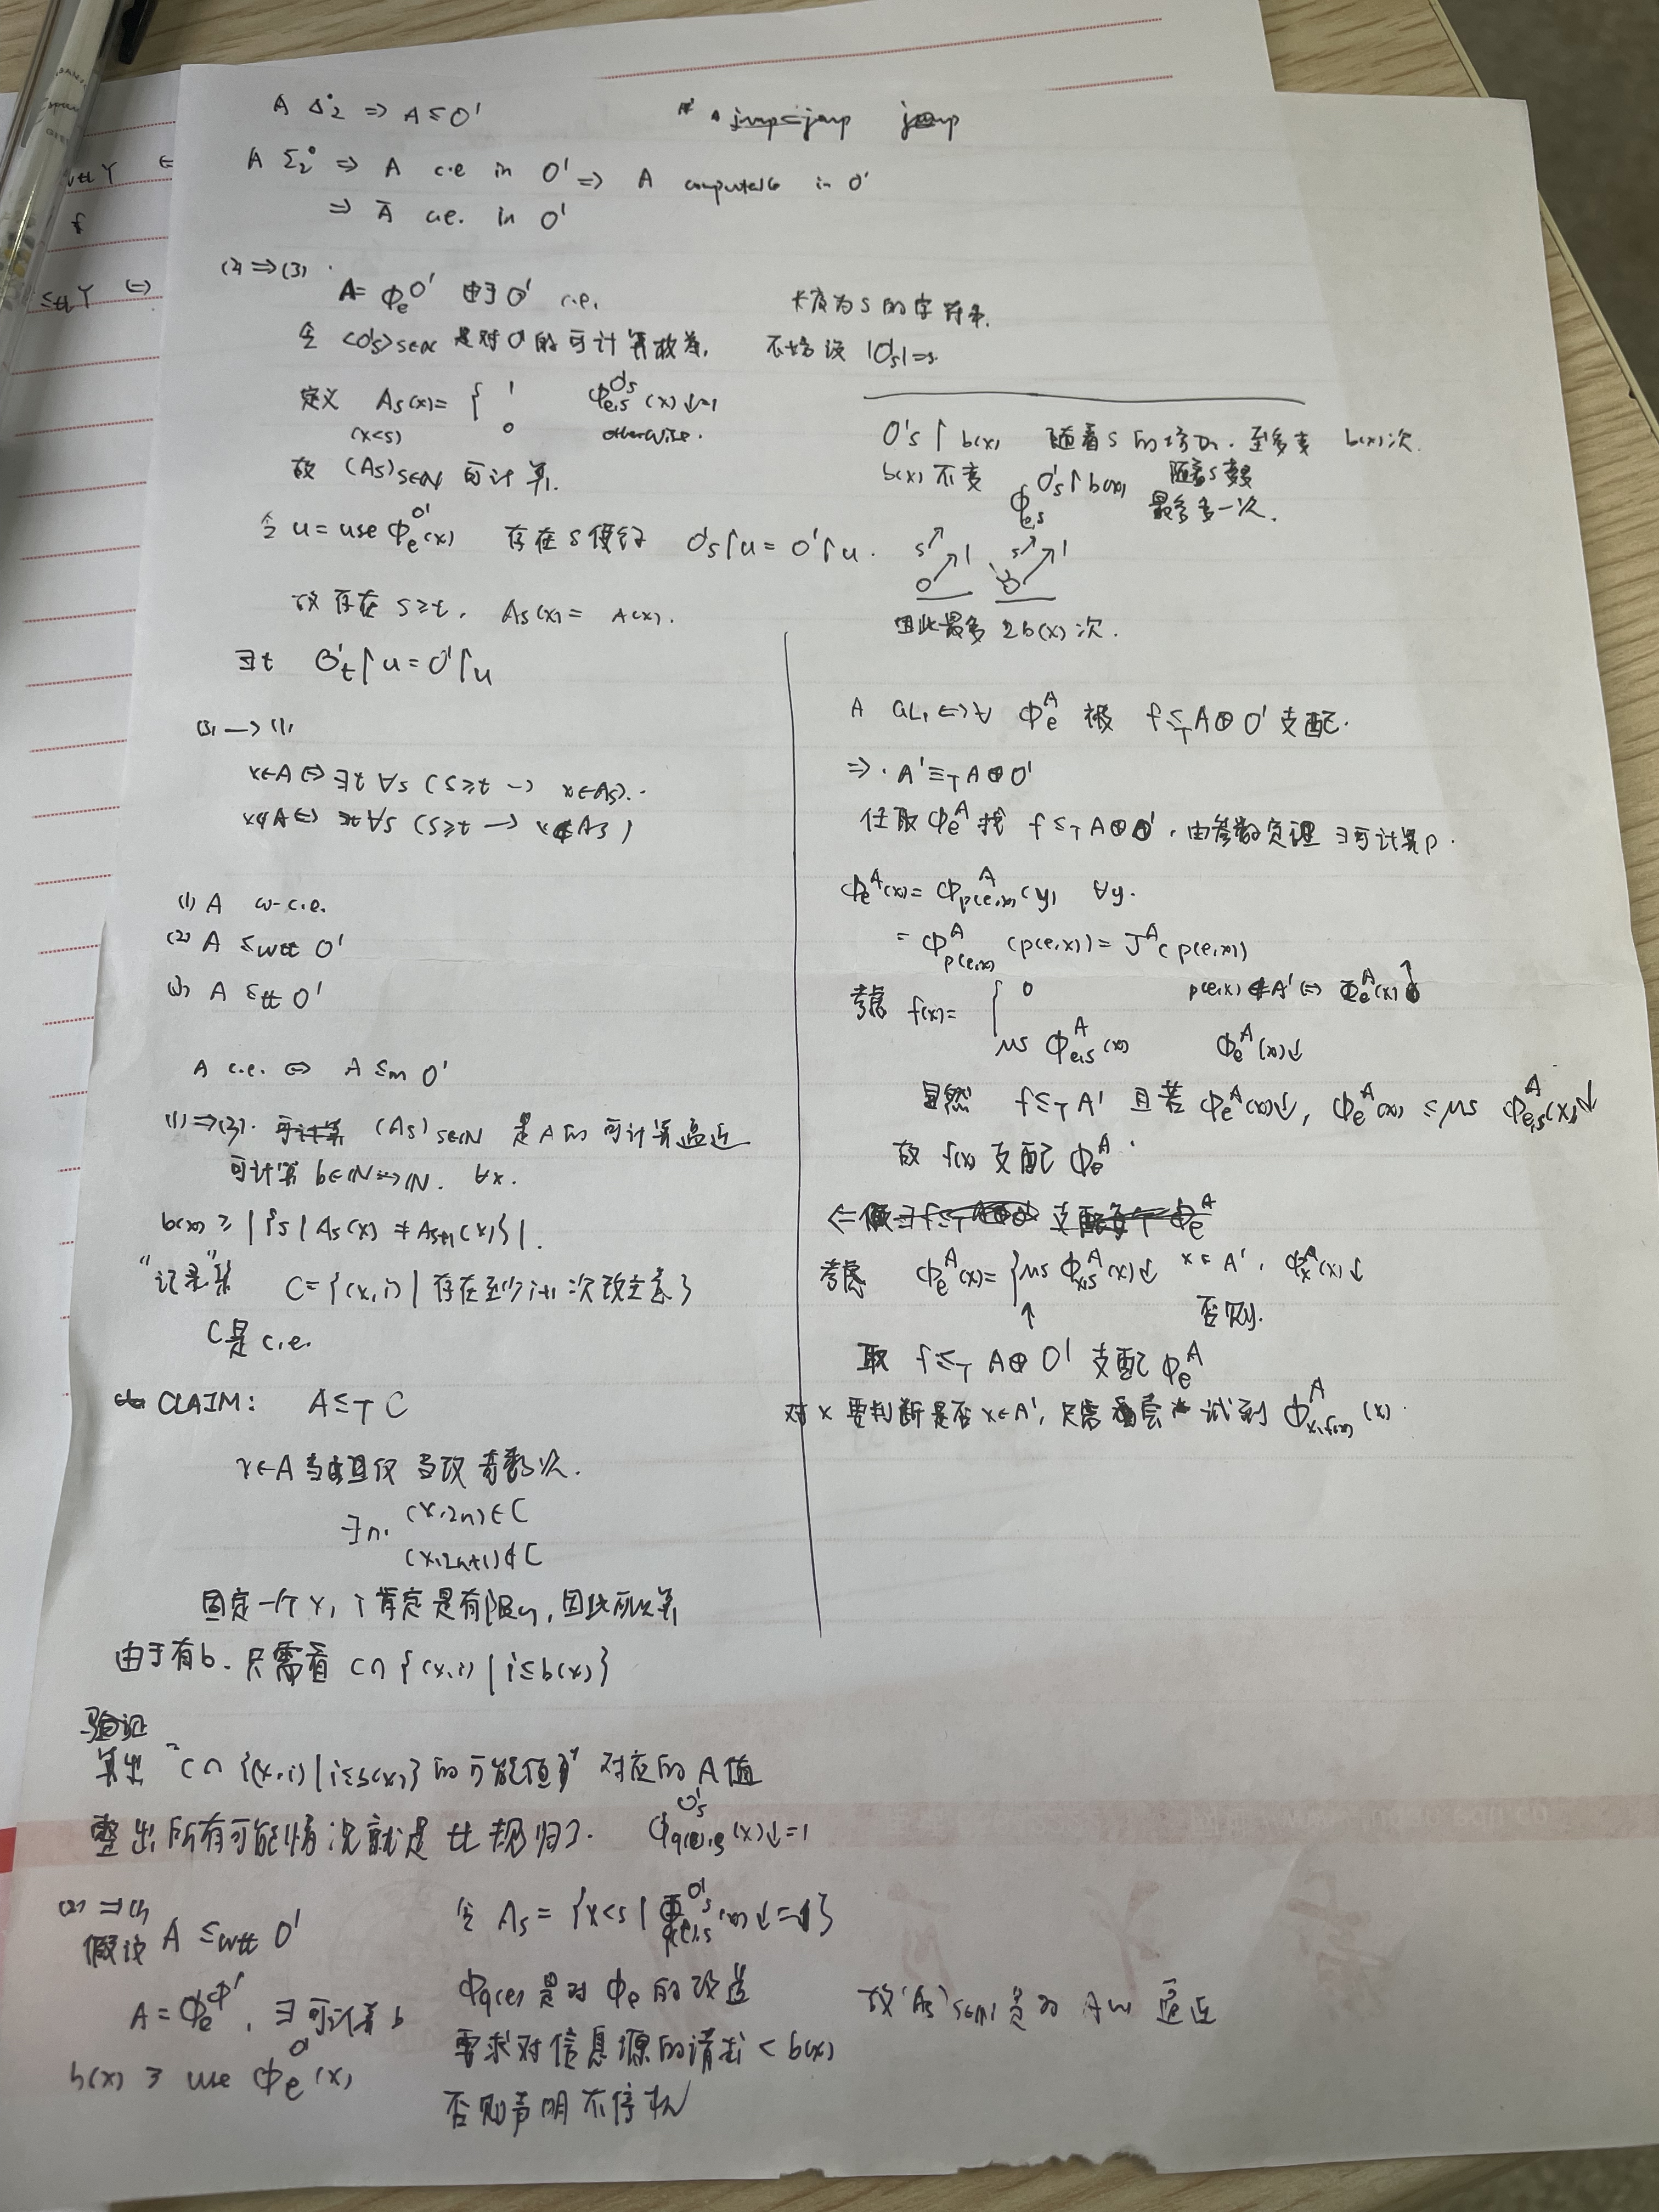
\includegraphics[width=.8\textwidth]{../images/ddia/1.jpg}
\captionof{figure}{\label{}A write conflict caused by two leaders concurrently updating the smae record}
\end{center}
\begin{enumerate}
\item Synchronous versus  asynchronous conflict detection
\label{sec:org47a8931}
In a multi-leader setup, both writes are successful, and the conflict is only detected
asynchronously at some later

You could make the conflict detetion synchronous - i.e., wait for the write to be replicated to
all replicas before telling the user that the write was successfull. However, by doing so, you
would lose the main advantage of multi-leader replication: allowing each replica to accept
writes independently.
\item Conflict avoidance
\label{sec:org7073fbf}
\item Converging toward a consistent state
\label{sec:orgf8914d7}
\item Custom conflict resolution logic
\label{sec:orgb569b14}
\end{enumerate}
\subsubsection{Multi-Leader Replication Toplogies}
\label{sec:orgfdbe32c}
\begin{center}
\includegraphics[width=.9\textwidth]{../images/ddia/2.jpg}
\captionof{figure}{\label{}Three example topologies in which multi-leader replication can be set up}
\end{center}

A problem with circular and star topologies is that if just one node fails, it can interrupt the
flow of replication messages between other nodes, causing them to be unable to communicate until
the node is fixed.

All-to-all topoligies can have issues. In particular, some network links may be faster than
others.
\begin{center}
\includegraphics[width=.9\textwidth]{../images/ddia/3.jpg}
\captionof{figure}{\label{}With multi-leader replication, writes may arrive in the wrong order at some replicas}
\end{center}

This is a problem of causality. To order these events correctly, a technique called \textbf{version vectors} can be used.
\subsection{Leaderless Replication}
\label{sec:org224d1ee}
\subsubsection{Leaderless Replication}
\label{sec:orge822084}
\end{document}